\clearpage
\section{What is life? Thinking quantitatively about living systems}
\label{sec:life}
% EDITORIAL ADDITION: navigation or conceptual bridge
The opening questions concern what makes a system living and what a physical explanation can reveal.
Order-of-magnitude thinking then turns broad questions into quantities that can be estimated and compared.
% Source: day4.tex:43; unit d4.2.0
\label{sec:life-features}
A useful thought experiment is to ask which properties of life on Earth might be universal and which might simply be particular implementations that arose on Earth.
If life existed elsewhere, some of its organizing principles might be recognizable even if its molecular details were completely different.

\begin{table}[h!]
\centering
\renewcommand{\arraystretch}{1.4}
\begin{tabularx}{0.9\textwidth}{
    |>{\raggedright\arraybackslash}X
    |>{\raggedright\arraybackslash}X|
}
\hline
\textbf{Potentially general feature} & \textbf{Earth-specific implementation that need not be universal}
\\
\hline
A self-replicating blueprint & DNA and its particular molecular structure
\\
\hline
Organization into self-replicating units & Cells as we know them
\\
\hline
Metabolism and energy transduction & Glycolysis, ATP, and particular terrestrial metabolic pathways
\\
\hline
Adaptation and/or evolution & Particular terrestrial evolutionary mechanisms and molecular machinery
\\
\hline
Birth and death of individual systems & Particular cellular life cycles
\\
\hline
A chemical basis for structure and function & CHNOPS chemistry
\\
\hline
Error correction and maintenance of information & Particular DNA-repair and proofreading mechanisms
\\
\hline
\end{tabularx}
\caption{A thought experiment about which features of terrestrial life might reflect general principles of living systems and which may be contingent molecular implementations.}
\end{table}


% ============================================================

% % Source: day4.tex:87; unit d4.2.1
% \subsection{The secrets of life}
% \label{sec:secrets}

% ============================================================

The phrase ``the secret of life'' became associated with the discovery of the structure of DNA through a famous anecdote.
According to James Watson's later account, after he and Francis Crick arrived at their double-helix model in 1953, Crick went into the Eagle pub in Cambridge and announced that they had ``found the secret of life'' \cite{watson2003dna}.
Their model suggested how genetic information could be copied through complementary base pairing \cite{watson1953molecular,watson1993genetical}.

About a decade later, Jacques Monod reportedly used the same language when he said to his colleague Agnes Ullmann, ``I think I have discovered the second secret of life'': allostery \cite{ullmann2011memoriam}.
Allostery is functional coupling between distinct sites on a protein, such that binding at one site changes binding or activity at another \cite{fenton2008allostery}.
We revisit allostery in section~\ref{sec:allostery}.
% Source: day1.tex:19; unit d1.1
\subsection{The scale of things: order-of-magnitude and Fermi thinking}
\label{sec:scale}


% ====================

Order-of-magnitude estimates and Fermi problems use a small number of known scales and physical constraints to obtain approximate answers to biological questions \cite{phillips2009feeling}.
When a quantity is known only to lie somewhere between two scales,
$x_{\min}$ and $x_{\max}$, a useful order-of-magnitude estimate is the geometric mean,

\[
    x_{\mathrm{est}} \sim \sqrt{x_{\min}x_{\max}}.
\]

This is especially natural when the uncertainty spans orders of magnitude.
On a logarithmic scale,

\[
    \log x_{\mathrm{est}} = \frac{1}{2} \left( \log x_{\min} + \log x_{\max} \right),
\]

so the estimate lies halfway between the two bounds in log-space.

\paragraph{Units and dimensional consistency}
Quantities that are added or equated must have the same dimensions.
For example, in the relation $\ell=vt$, the distance $\ell$ has dimensions of length, so the velocity $v$ must have dimensions of length divided by time.
Arguments of exponential, logarithmic, and trigonometric functions must be dimensionless.
Thus, in an exponential decay $e^{-t/\tau}$, the characteristic timescale $\tau$ must have the same units as $t$, making the ratio $t/\tau$ dimensionless.

Dimensional reasoning can also identify a characteristic scale before a detailed calculation.
The diffusion constant has dimensions
\[
    [D]=\frac{\text{length}^2}{\text{time}}.
\]
The characteristic time constructed from a length $\ell$ and a diffusion constant $D$ is therefore $t_D\sim\ell^2/D$.
For $\ell=10\,\mu\mathrm{m}$ and $D=1\,\mu\mathrm{m}^2\mathrm{s}^{-1}$, this gives $t_D\sim100\,\mathrm{s}$.
The numerical prefactor depends on the dimension, geometry, and precise meaning of ``diffuse across.''

\paragraph{A practical Fermi-estimation protocol}
\begin{enumerate}
    \item State the quantity and its desired units.
    \item Decompose it into factors that can be estimated.
    \item Assign a plausible scale to each factor.
    \item Multiply, keeping powers of ten and units explicit.
    \item Check the result against obvious lower and upper bounds.
    \item Report the assumptions and only the precision justified by the estimate.
\end{enumerate}

As an illustrative estimate, take deliberately rounded bacterial-scale values: a ribosome adds roughly $20$ amino acids per second, a typical protein contains roughly $300$ amino acids, approximately $10$ ribosomes translate one mRNA simultaneously, and the mRNA has an effective lifetime of about five minutes.
These values are representative rather than universal.
% compare BioNumbers entries BNID~100059, BNID~108985, BNID~105001, and BNID~111927 \cite{milo2010bionumbers}.
One ribosome completes a protein in approximately $300/20\sim15\,\mathrm{s}$, so ten ribosomes produce of order $10/15\sim0.7$ proteins per second.
Over this five-minute timescale, this gives roughly $0.7\times300\sim200$ proteins.
The point is the scale and the assumptions, not a falsely precise value.
Further biological examples and experimentally measured scales are collected in the BioNumbers database \cite{milo2010bionumbers}, and are also available at \href{https://book.bionumbers.org}{book.bionumbers.org}.
% Source: day1.tex:42; unit d1.2


\subsection{Case study: inferring a lipid bilayer from areas}
\label{sec:gorter}


% ====================

Gorter and Grendel used red blood cells to infer that cellular membranes
consist of a lipid bilayer \cite{gorter1925bimolecular}.

The basic logic was:

\begin{enumerate}
    \item Take a known number of red blood cells.
    \item Estimate the total surface area of those cells.
    \item Extract the lipids from the cells.
    \item Spread the extracted lipids into a monolayer.
    \item Measure the area occupied by this lipid monolayer.
\end{enumerate}

The lipid monolayer occupied approximately twice the area of the cell
surfaces. This suggests that the membrane contains two layers of lipid:

\[
    A_{\mathrm{lipid}} \approx 2 A_{\mathrm{cell}}.
\]

Hence the membrane is approximately a lipid bilayer.

% \cs{ \href{https://link.springer.com/chapter/10.1007/978-981-10-6823-2_2}{insert figure from this paper}}

\begin{figure}[h]
    \centering
    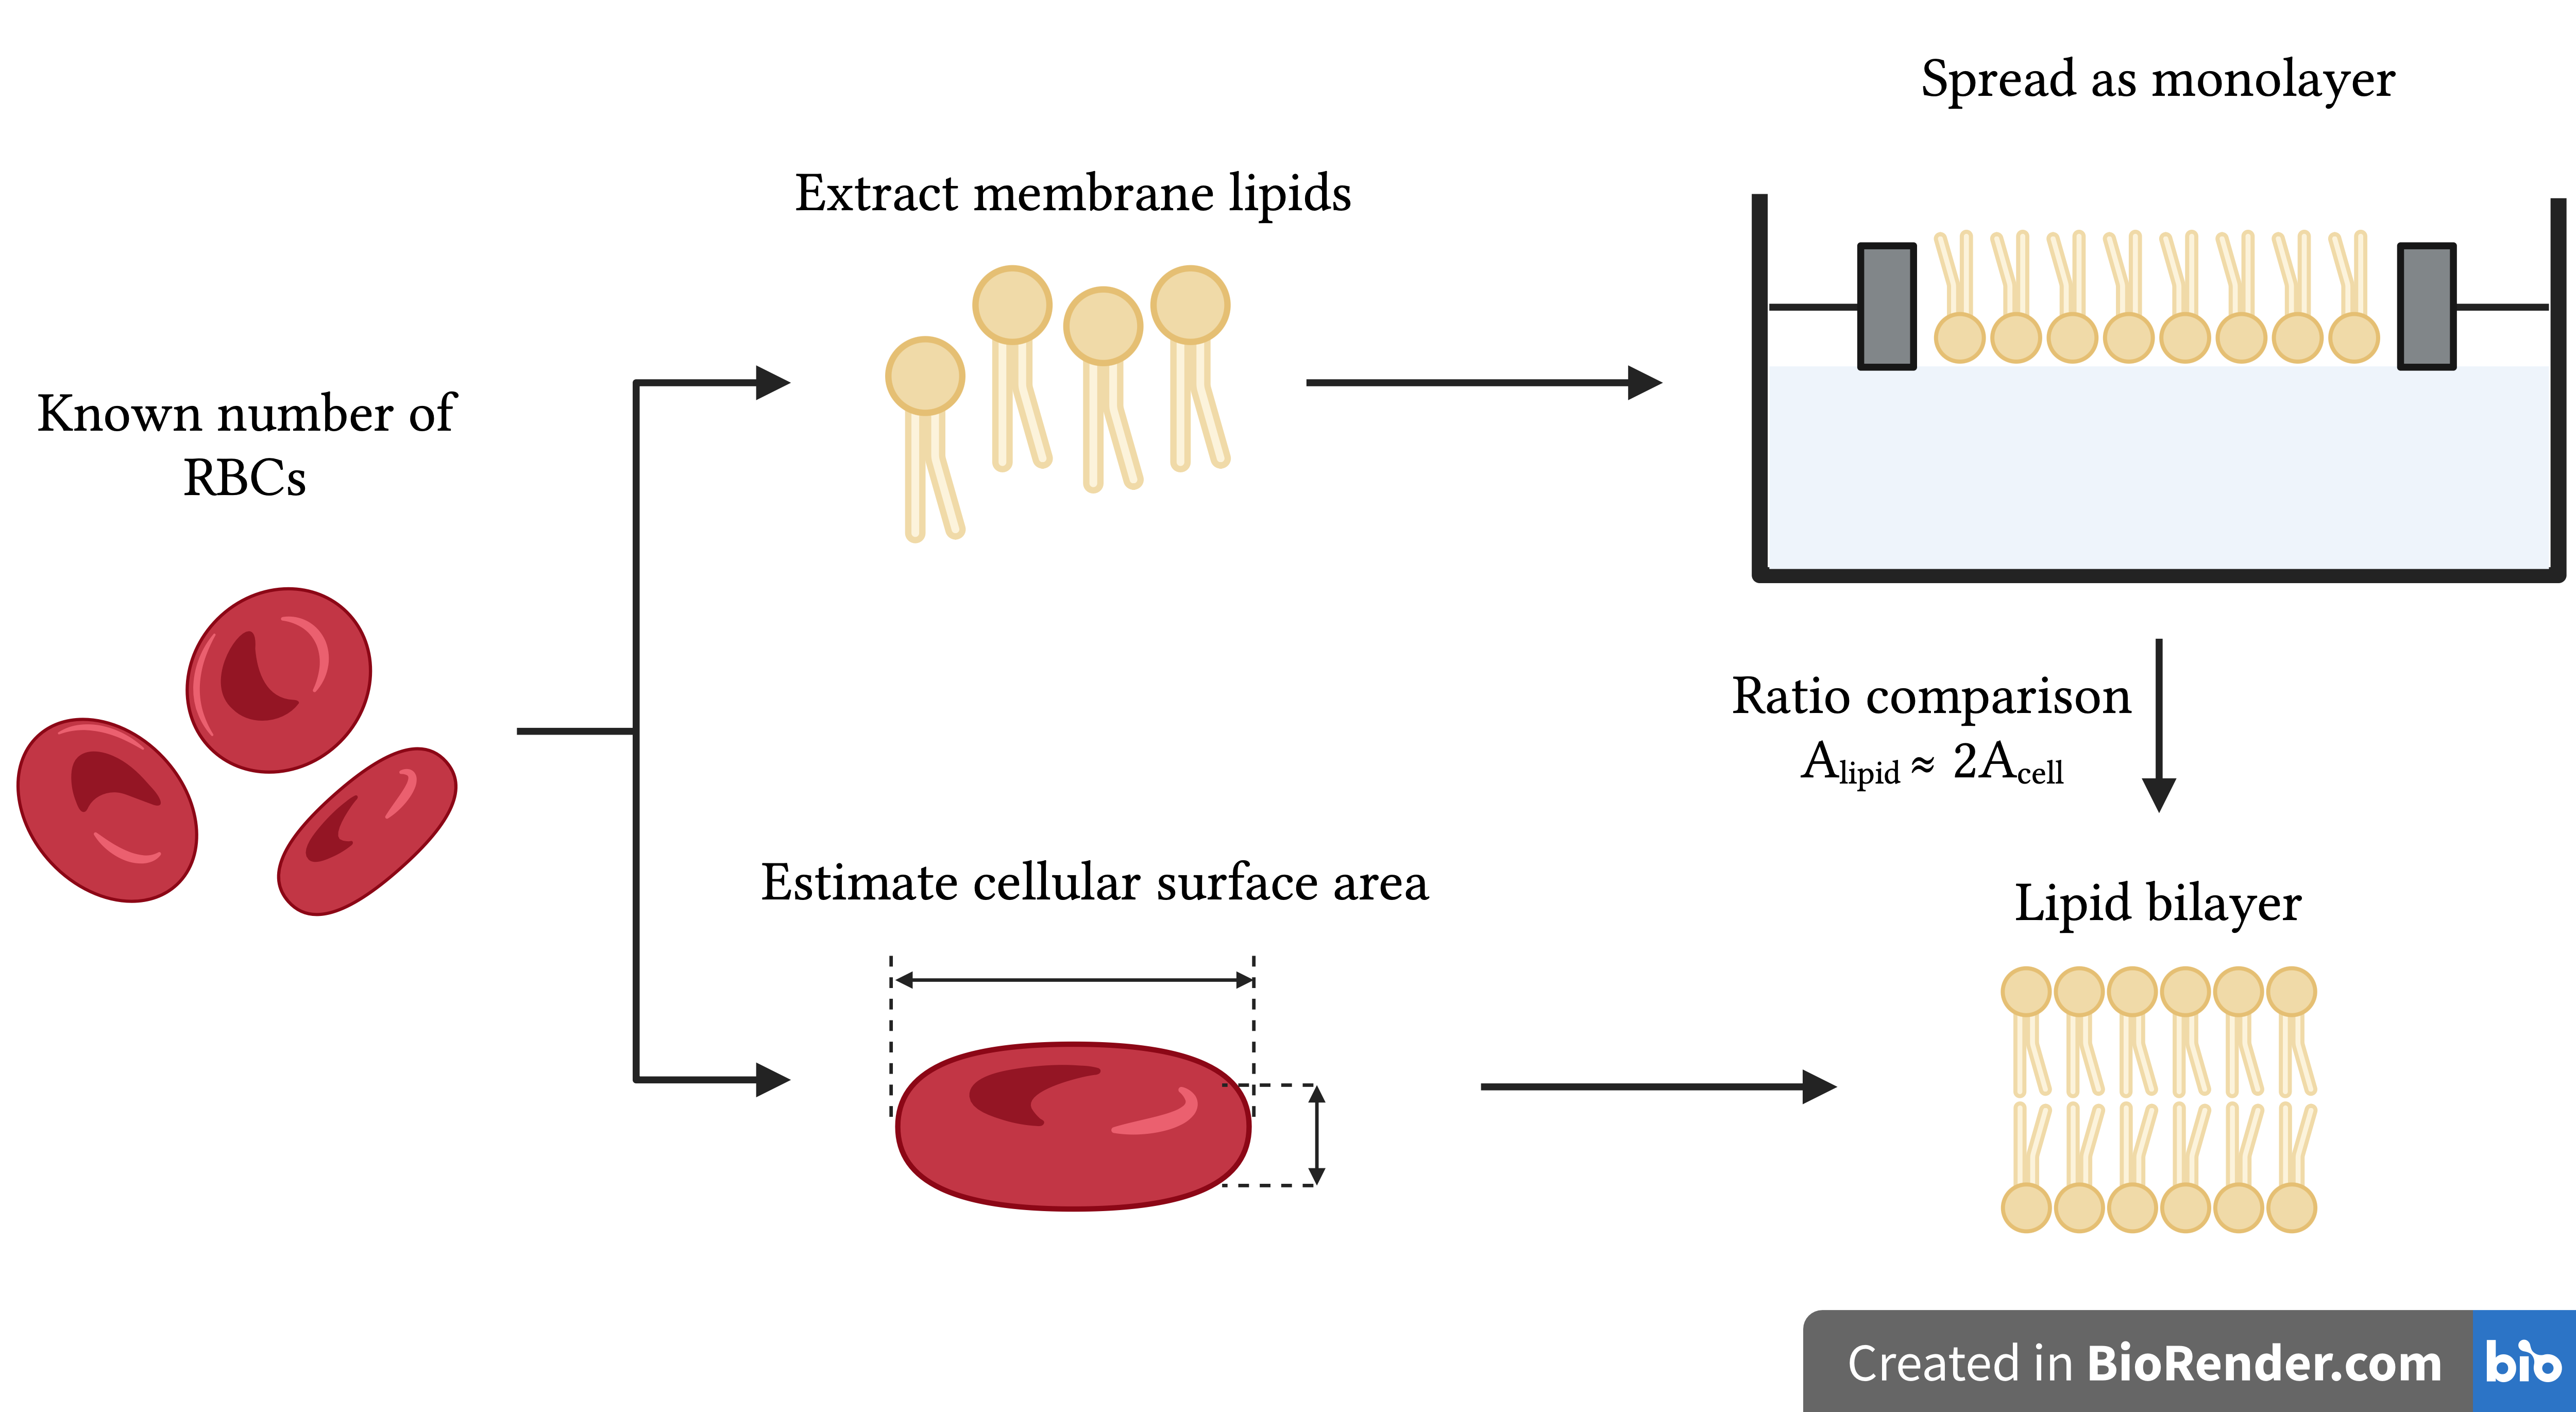
\includegraphics[width=0.8\linewidth]{../figures/gorter_grendel.png}
    \caption{The Gorter-Grendel experiment \cite{gorter1925bimolecular}.
    Lipids extracted from a known number of red blood cells were spread into a monolayer and compared with the estimated total surface area of the cells.
    The lipid monolayer occupied approximately twice the cell-surface area, $A_{\mathrm{lipid}}\approx 2A_{\mathrm{cell}}$, providing evidence that the cell membrane consists of a lipid bilayer. Created with BioRender.com.}
    \label{fig:gorter-grendel}
\end{figure}

% ====================

